\Chapter{Introduction}
	\section{Fondamentaux de la physique des plasmas}
		 
		\emph{Le plasma}. Le plasma est souvent considéré un peu équivoquement
		comme le quatrième état de la matière. Dans notre environnement proche,
		nous avons pris conscience de son existence à travers les phénomènes de flammes,
		d'éclairs, d'aurore boréales ou d'arc électriques. Mais à des conditions de
		pressions et de températures différentes de celles de notre atmosphère
		terrestre, il est omniprésent : plus de 99\% de la matière connue est sous
		cette forme. 
		
		Une définition plus adaptée du plasma est celle d'un gaz conducteur. Une partie des
		atomes le composant est ionisée, dannant naissance à une population
		d'électrons libres et d'ions de différentes espèces. Ces populations permettent alors
		le transport de courant et, sensibles aux forces électromagnétiques, influencent
		fortement le comportement global du plasma en provoquant des phénomènes
		collectifs, non-linéaires et turbulents.
		
		Le plasma et son comportement sont décrits par la théorie de la physique des
		plasmas. Elle intègre les connaissances de nombreux domaines, tels que la
		physique statitique, l'électromagnétisme, ou encore la dynamique des fluides.
		
		\subsection{Les paramètres plasmas}
		
			Les plasmas se définissent donc comme des gaz possédant une population
			d'électrons libres $n_e$ à une température électronique $T_e$. 
			La figure \ref{zoologie} issue de \cite{national1995Plasma}
			représente une classification des plasmas en fonction de ces deux paramètres 
			principaux qui vont influer sur la dynamique du transport de courant.
			La théorie présentée dans la suite de cette thèse ne concerne que les plasmas
			dits classiques :
			\begin{itemize}
			  \item les plasmas naturels peu dense tels que l'espace interstellaire,
			  le vent solaire, la magnétosphère, et l'ionosphère
			  \item les plasmas naturels denses tels que les éclairs et les étoiles
			  \item les plasmas industriels, de laboratoire, et thermonucléaires
			\end{itemize}
			\begin{figure}[h]
				\centering
				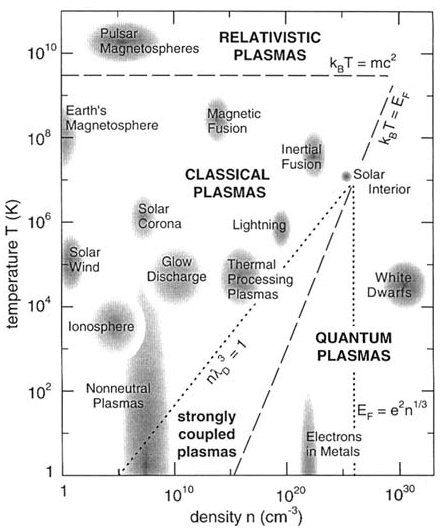
\includegraphics[height=100mm,width=80mm]{figures/zoologie.png}{\caption{Classification
				de différents plasmas en fonction de $n_e$ et $T_e$.}\label{zoologie}}
			\end{figure}
			
			Dans ces plasmas, le dégré d'ionisation $\alpha$ est donné par le rapport
			entre la densité électronique $n_e$ et la densité de gaz $n_g$ :
				$$\alpha=\frac{n_e}{n_e+n_g}$$
			Cette fraction va définir l'importance de l'interaction entre les particules 
			neutres et les particules chargées. Même à très faible $\alpha$, l'apparition
			d'une population de porteurs de charge va modifier les caractéristiques et la
			dynamique du plasma. 
			
			L'ionisation du gaz suit l'évolution de la température électronique $T_e$ qui
			mesure l'agitation thermique des électrons. Densité et température
			électronique permettent de définir le paramètre plasma\footnote{Le
			paramètre plasma représente le ratio entre l'énergie thermique des électrons
			et leur énergie potentielle electrostatique coulombienne \emph{ie.}
			l'agitation thermique desordonnée contre les forces d'interactions
			coulombiennes structurantes.}:
				$$\Gamma=\frac{<E_p>}{<E_c>}=\frac{e^2n_e^{1/3}}{\epsilon_0 kT_e}$$
			Les plasmas classiques sont caractérisés par $\Gamma\ll 1$. Ils ont une
			population d'électrons assez espacée et/ou une température suffisamment élevée. 
			
		\subsection{Echelles, phénomènes collectifs et collisions}
			Le plasma est un milieu très complexe où de multiples dynamiques interfèrent. 
			Au milieu du gaz en équilibre thermique, les ions et les électrons issus
			de l'ionisation se réorganisent spatialement pour minimiser les forces
			de Coulombs ($\mathbf F=q\mathbf E$) et de Laplace ($\mathbf F=-q\mathbf
			B\times\mathbf v$) qui se forment dans le système et rendre l'ensemble
			électriquement neutre. Le plasma est dans un état de \emph{quasi-neutralité}, 
			\ie vu de suffisement loin et exepté à ses frontières, $n_e=n_i$.
			
			
		 Plasma parameter $\Lambda$ Debye sphere, Quasineutrality Debye length,
		Electrostatic plasma frequency $\omega_c$
		 Density : Degree of ionisation $\alpha=n_i/(n_i+n_n)$
			Temperature : Saha equation, thermal equilibrium, Maxwellian energy dist function
			Potentials : Debye sheath, Boltzmann relation
			Magnetization : Hall parameter, Larmor radius, plasma frequency
		
	\section{Fluid description of a plasma}
	\lipsum{50}
		\subsection{Statistical description}
			\subsubsection{BBGKY hierarchy, liouville equation}
			\subsubsection{The Boltzmann equation}
			\lipsum{50}
		\subsection{Moments of the Boltzmann equation, conservation laws}
			Braginskii equations
			\subsubsection{Continuity equation}
			\lipsum{50}
			\subsubsection{Momentum equation}
			\lipsum{50}
			\subsubsection{Energy equation}
			\lipsum{50}
			\subsubsection{Heat equation}
			\lipsum{50}
	\section{Low-temperature plasmas}
		\subsection{Creation of the discharge, role of electrons}
		Dans les plasmas basse-température industriels et de laboratoires, qui possédent
			un faible degré d'ionisation, ou dans l'ionospère, la dynamique du plasma est dominée par
			la perte de quantité de mouvement dûe à l'ionisation la force de friction avec le gaz.
		Electrical breakdown, Townsend avalanche, 
		\lipsum{50}
		\subsection{Ions transport and ambipolar field}
	\section{Edge plasma physics of tokamaks}
		Lawson criteriom, strongly magnetized
		\subsection{Fusion and tokamaks}
		\subsection{Drift velocities}
		\subsection{Turbulence and anomalous transverse transport}
		\lipsum{50}
	\section{Plasma surface interaction and sheath physics}
		\lipsum{50}
		\subsection{Debye sheath}
			\lipsum{50}
		\subsection{Bohm criterium}
			\lipsum{50}
		\subsection{Open field line physics}
			\lipsum{50}
		\subsection{Issue of sheath parallel to the magnetic field}
			\lipsum{50}

		